\documentclass{article}
\usepackage[utf8]{inputenc}
\usepackage[T2A]{fontenc}
\usepackage[english,russian]{babel}
\usepackage[left=1.5cm,right=1.5cm,top=2cm,bottom=2cm]{geometry}
\usepackage{hyperref}
\usepackage{enumitem}
\usepackage{graphicx} %библиотека для графики и картинок
\DeclareGraphicsExtensions{.pdf,.png,.jpg}
\usepackage{listings}


\begin{document}
% НАЧАЛО ТИТУЛЬНОГО ЛИСТА
\begin{center}
    \Large
    Федеральное государственное автономное \\
    образовательное учреждение высшего образования \\ 
    «Национальный исследовательский университет ИТМО»\\
    \vspace{0.5cm}
    \large
    
    \vspace{1cm}
    \Large
    \textbf{По дисциплине «Информационная безопасность»} \\
        Лабораторная работа №4\\
        Анализ уязвимостей веб-приложения с
помощью OWASP ZAP
    \large
    \vspace{8cm}

    \begin{minipage}{.33\textwidth}
    \end{minipage}
    \hfill
    \begin{minipage}{.4\textwidth}
    
        \textbf{Студент}: \vspace{.1cm} \\
        \ Дениченко Александр Олегович P3412\\
        \textbf{Практик}:  \\
        \ Маркина Татьяна Анатольевна
    \end{minipage}
    \vfill
Санкт-Петербург\\ 2025 г.
\end{center}
\pagestyle{empty}
% КОНЕЦ ТИТУЛЬНОГО ЛИСТА 
\newpage
\pagestyle{plain}

\section*{Цель}

Освоить базовые навыки динамического тестирования безопасности (DAST) на
примере тестового приложения.

\section{Вводная часть}

Изначально был установлен OWASP ZAP и запущен. Выбран режим Quick Scan.
\\ \\
Для тестирования был выбран сайт \href{http://testaspnet.vulnweb.com}{http://testaspnet.vulnweb.com}. Данный сайт не является коммерческим, а является тестовым приложением для тестирования безопасности.
Не будет этично тестировать реальные сайты на уязвимости и баловаться с нагрузкой.

\section{Ход работы}

Изначально я перешёл на тестовый сайт во встроенном браузере ZAP. Выбрал режим Automatic Scan + поставил галочку, чтобы использовать традиционный Spider. Далее запустил атаку.

\begin{center}
  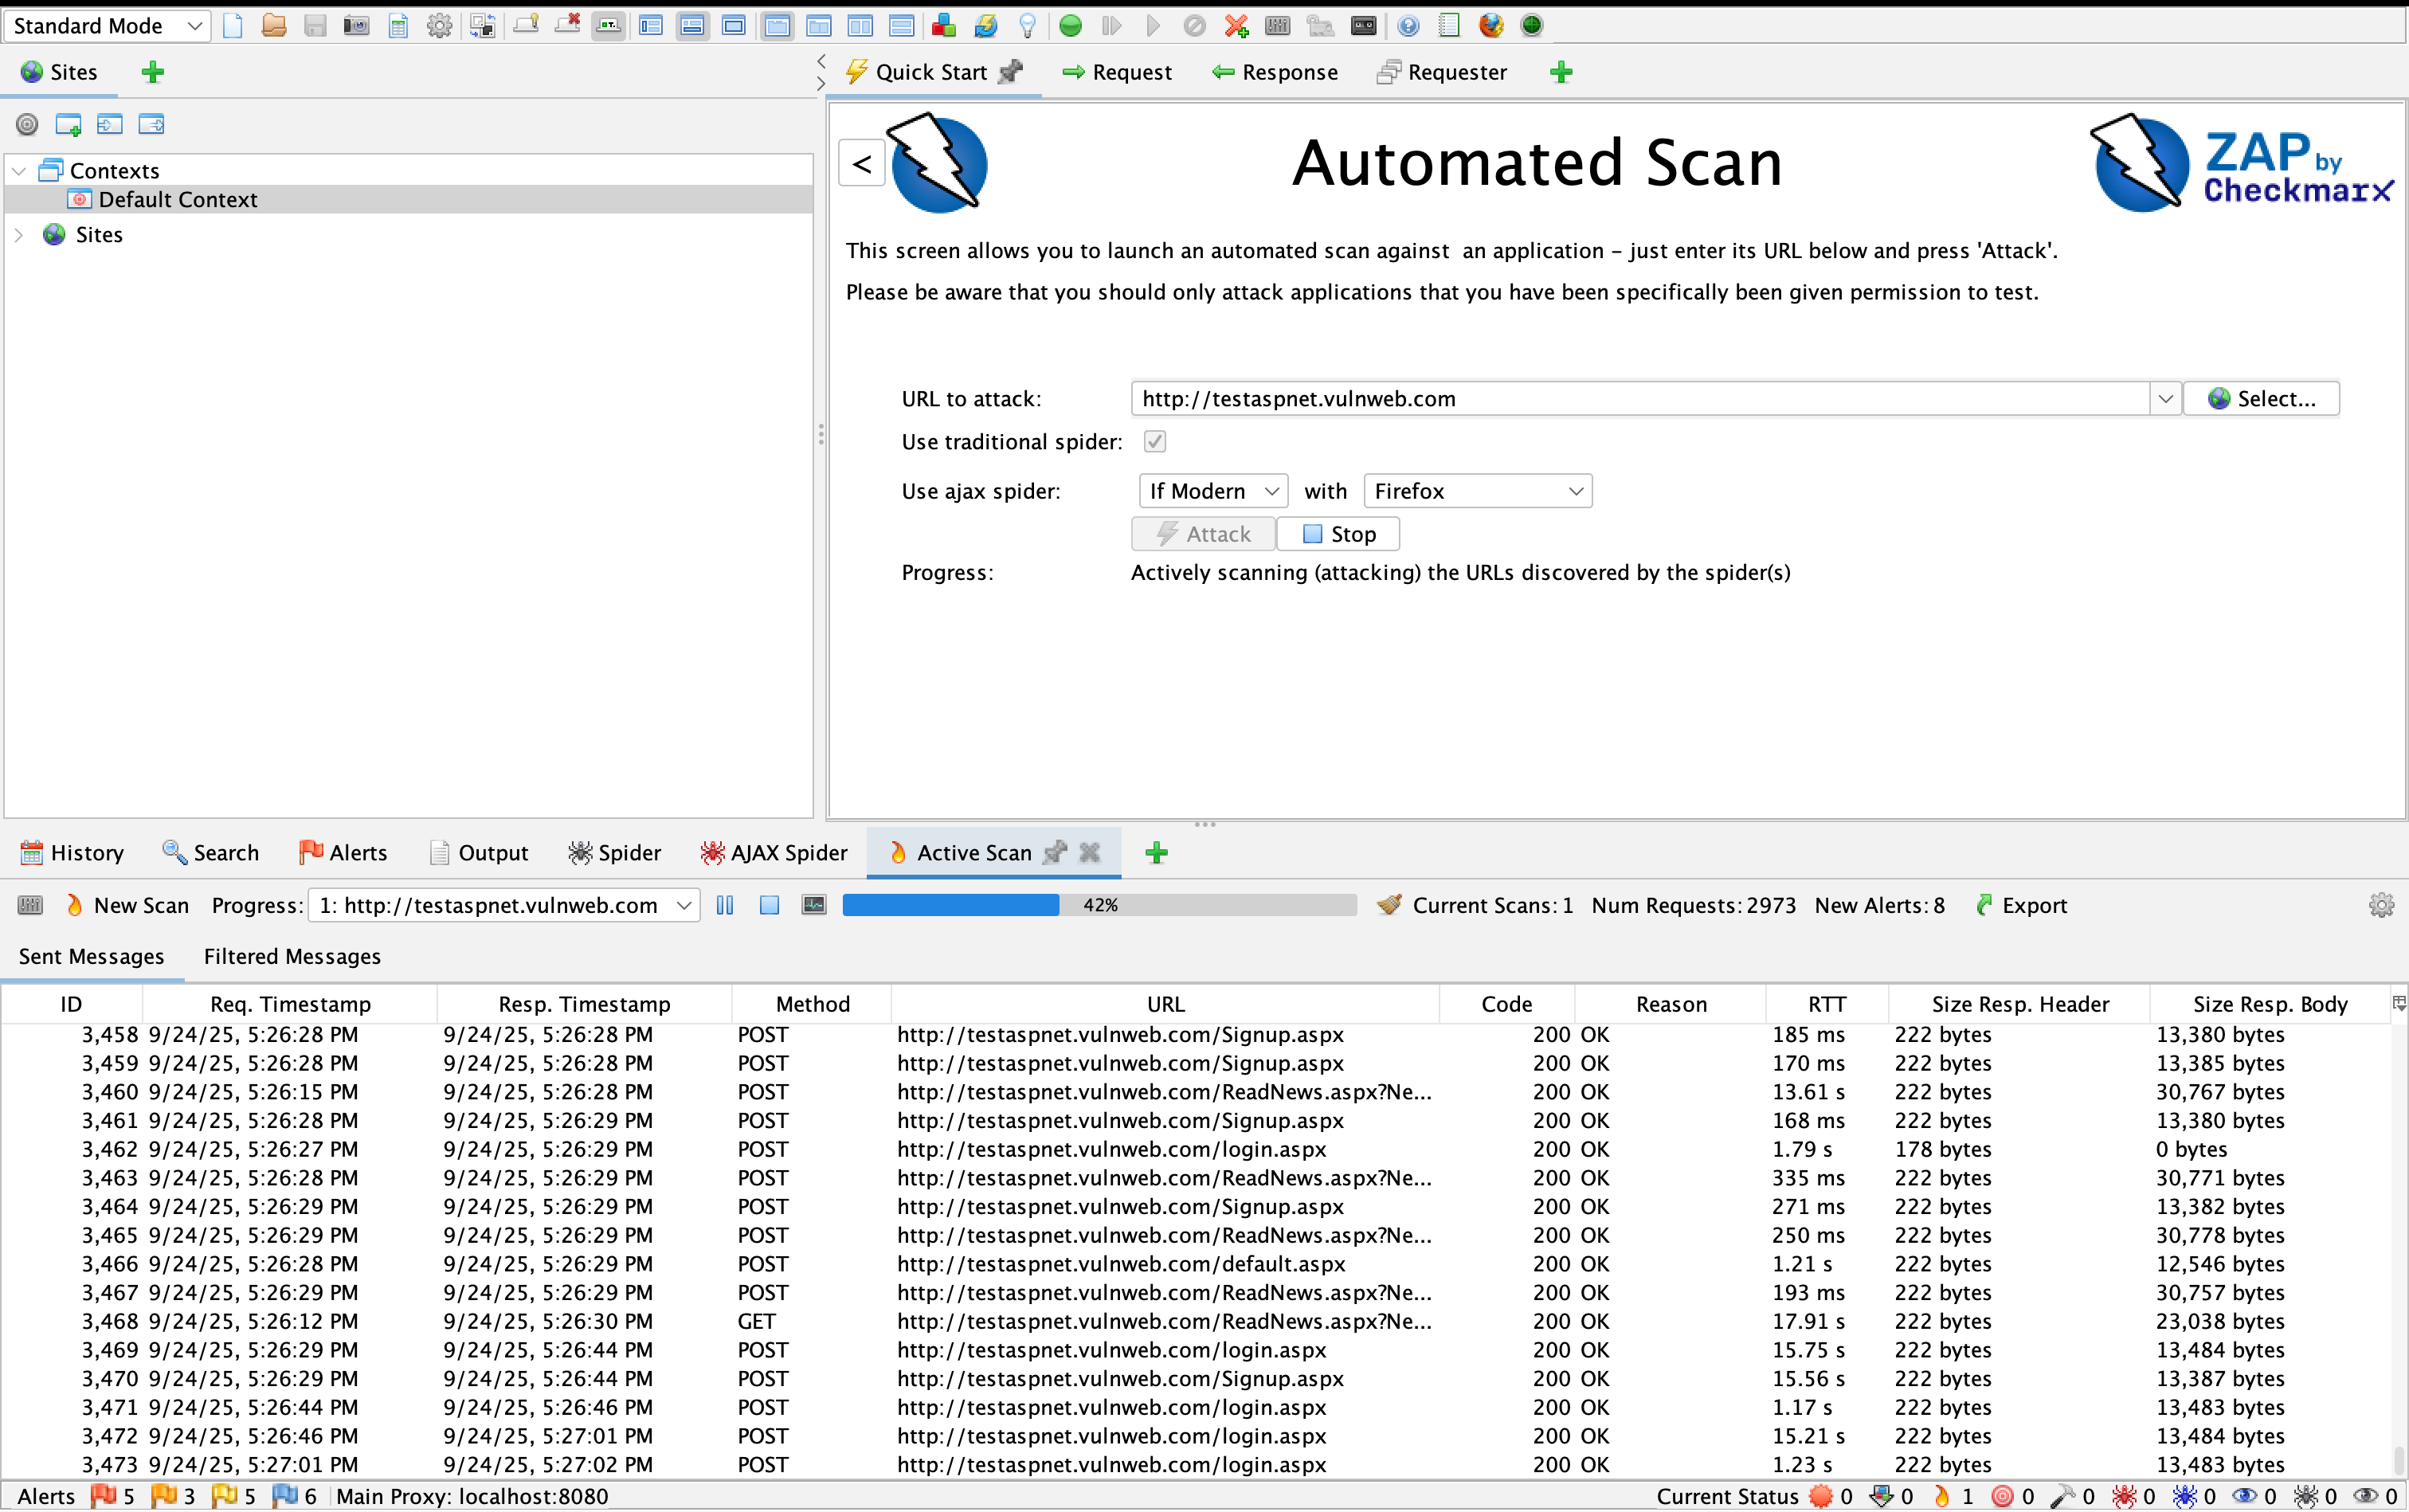
\includegraphics[width=.9\textwidth]{scan}
\end{center}

В течении сканирования выявлено 20 Alerts. 

\begin{center}
  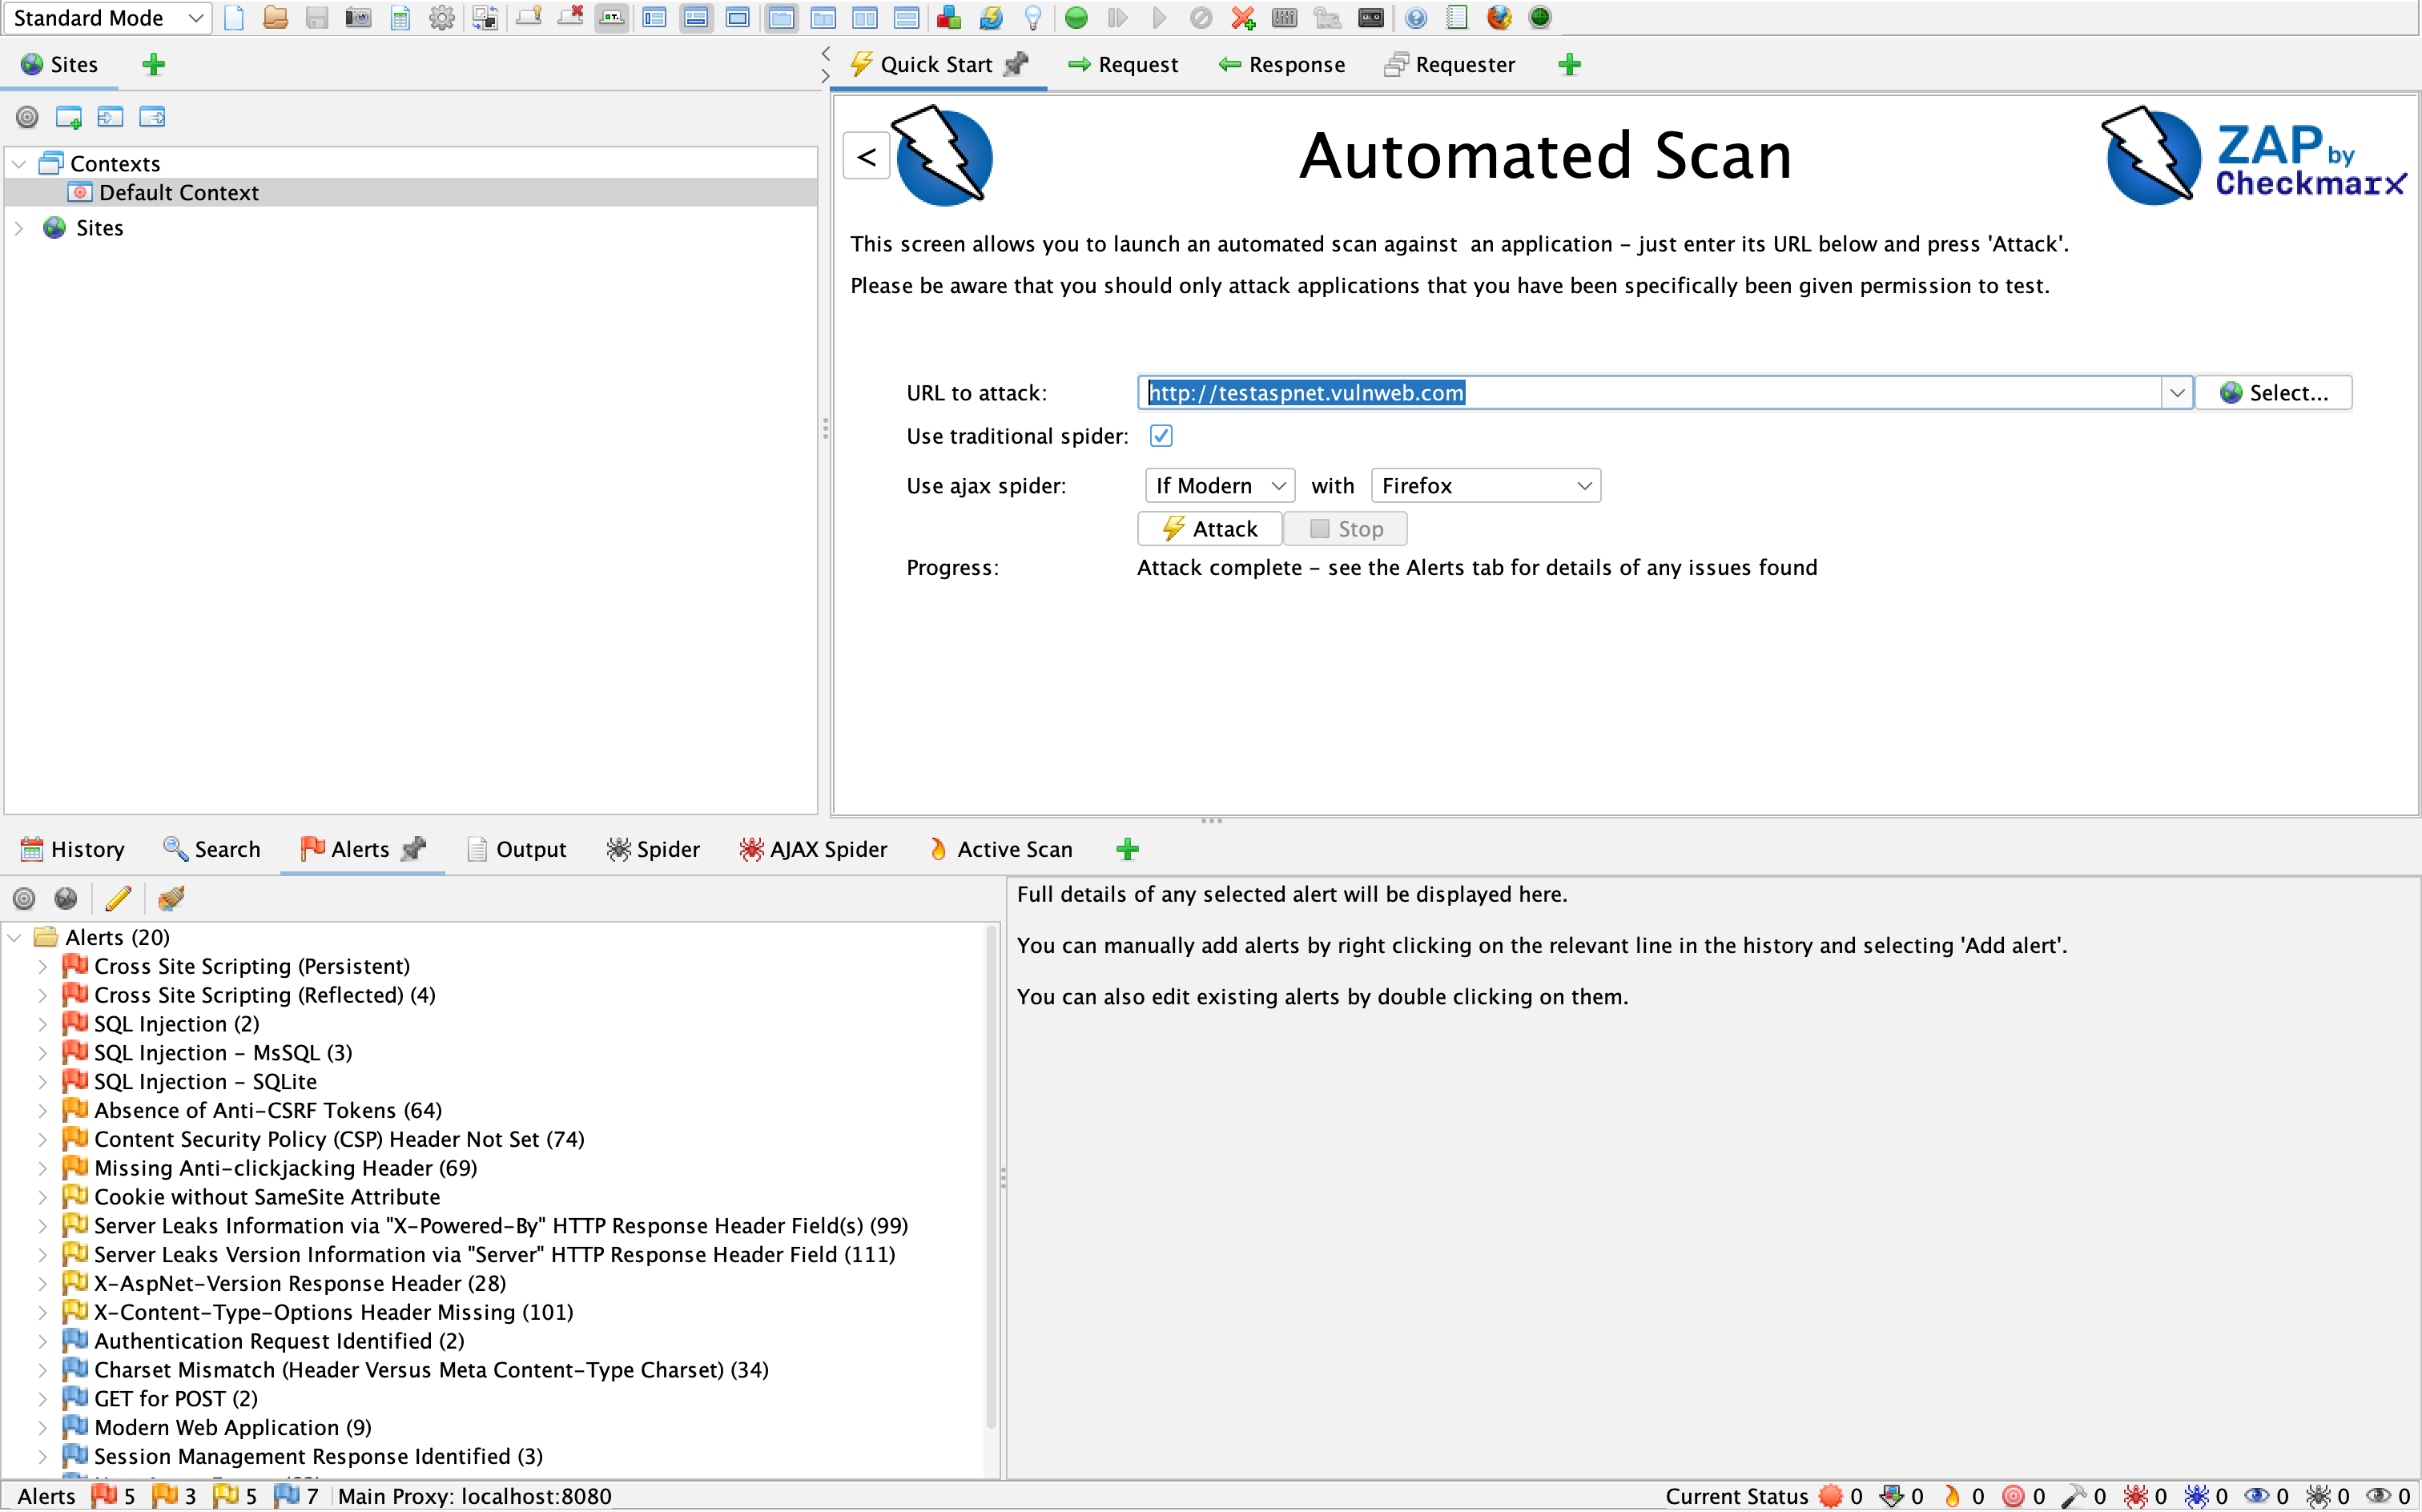
\includegraphics[width=.9\textwidth]{end}
\end{center}

По окончанию сканирования я сгенерировал отчёт и рассмотрел раздел Alerts.

\section{XSS}

\begin{center}
  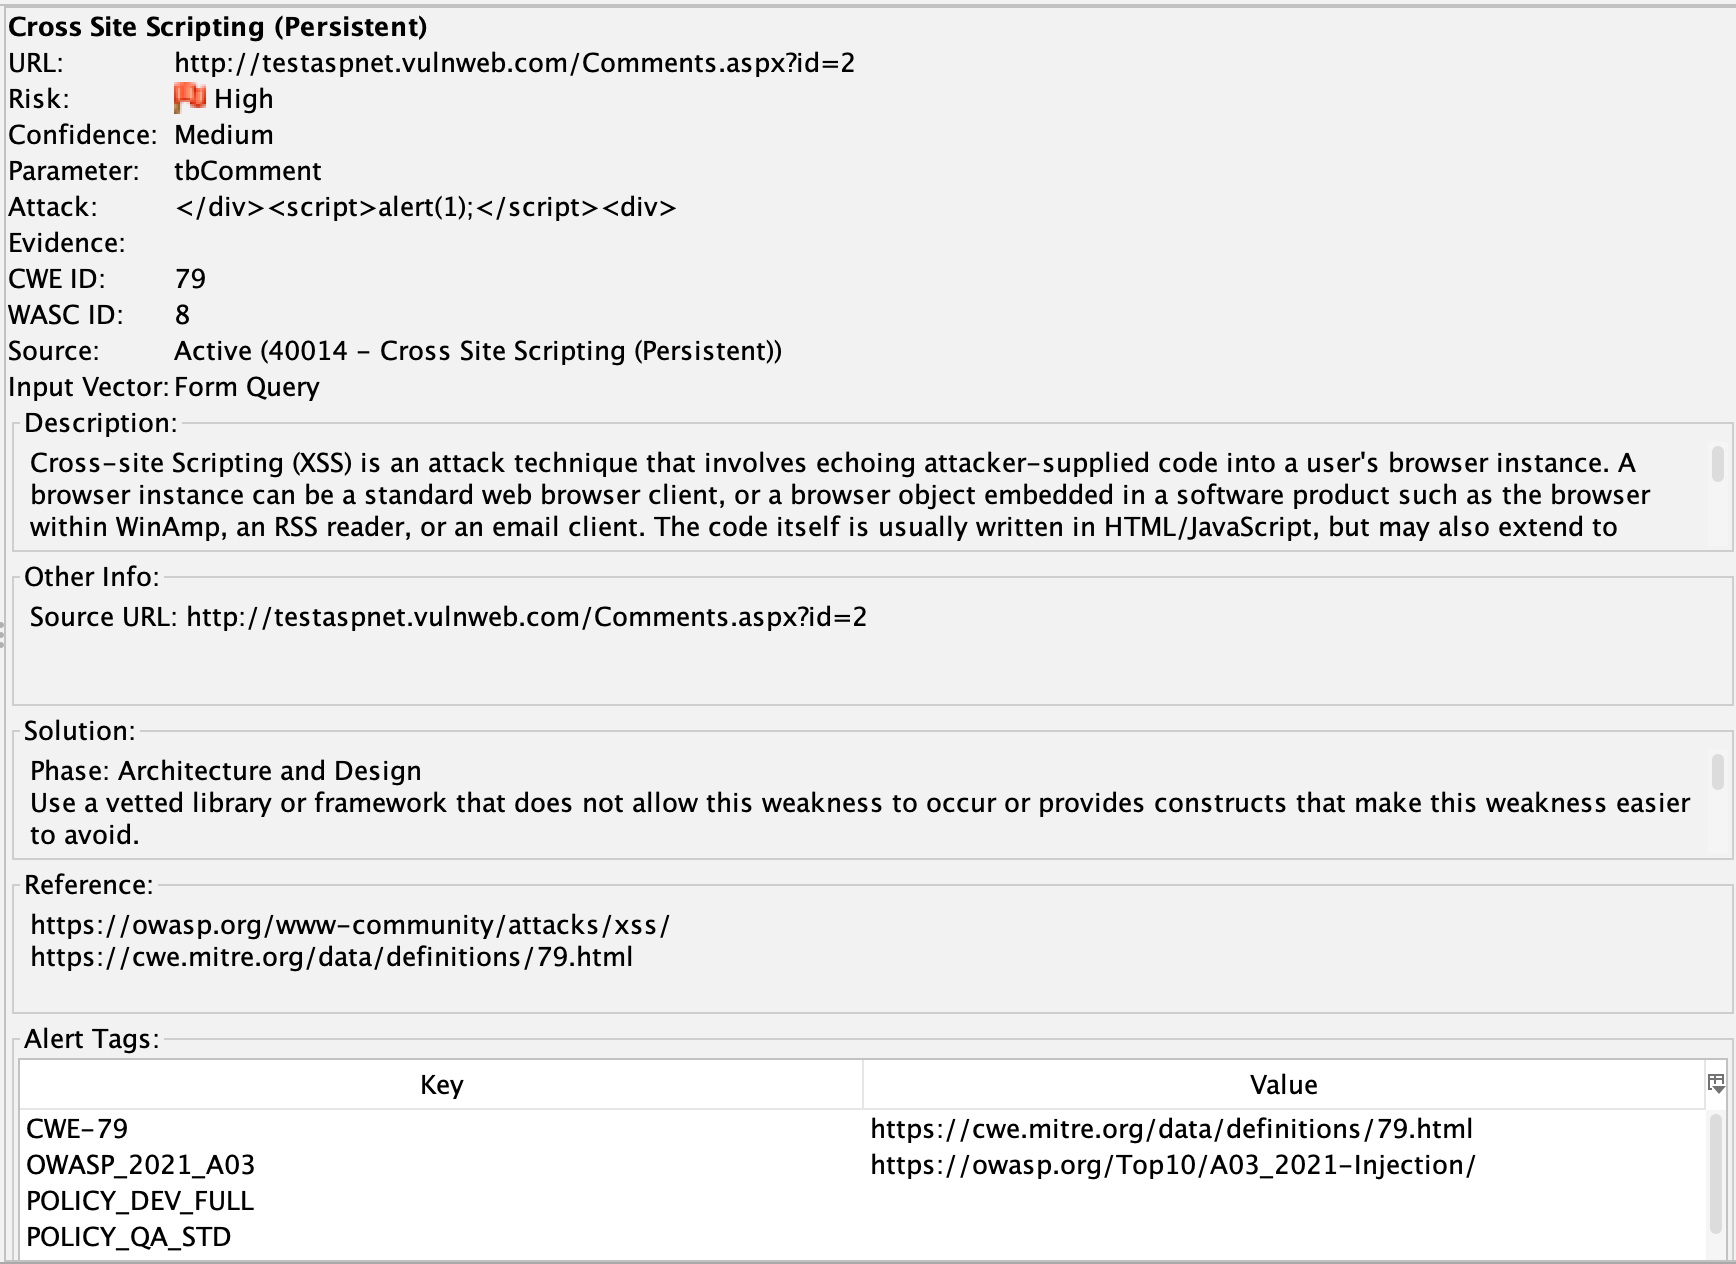
\includegraphics[width=.9\textwidth]{1}
\end{center}

Сканирование выявило критическую уязвимость: Persistent Cross Site Scripting (XSS) на странице комментариев по адресу http://testaspnet.vulnweb.com/Comments.aspx?id=2. Это позволяет злоумышленнику сохранять вредоносный скрипт, который будет выполняться для всех пользователей, просматривающих страницу.

Атака: внедрение кода через комментарий:
\begin{lstlisting}
  </div><script>alert(1);</script><div>
\end{lstlisting}

Уязвимость подтверждена как персистентная: скрипт сохраняется на сервере и срабатывает для любого пользователя. Уязвимости CWE-79 (OWASP TOP 10 — Injection).

% Для устранения применять "против XSS"-библиотеки и методы экранирования данных пользователем при выводе на страницу.

\begin{center}
  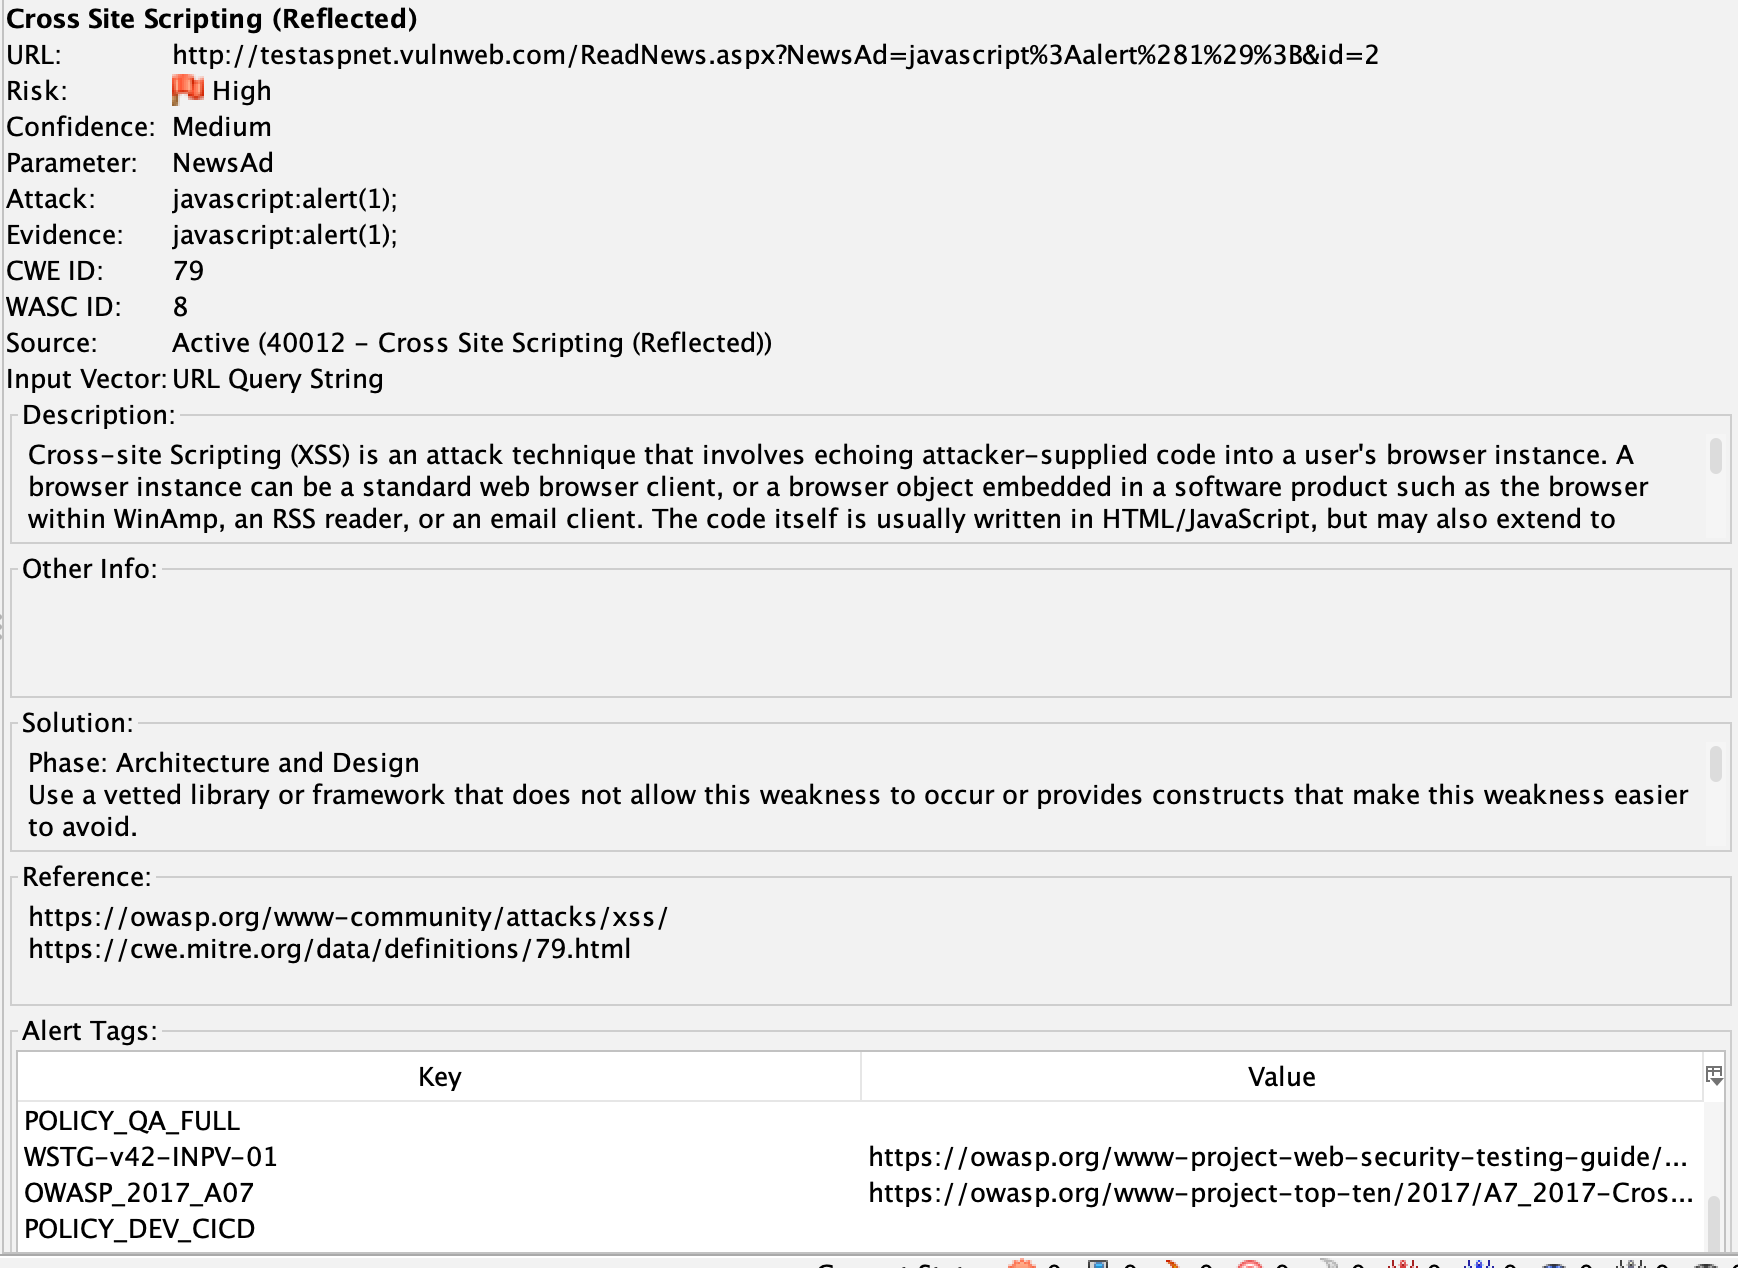
\includegraphics[width=.9\textwidth]{1-1}
\end{center}

Cross Site Scripting (Reflected) — отражённое межсайтовое выполнение скриптов (XSS). 

Данная XSS-уязвимость позволяет злоумышленнику внедрить и выполнить JavaScript-код на сайте через параметр URL, если жертва перейдёт по специально подготовленной ссылке. Скрипт выполняется немедленно после перехода и может привести к краже сессии, подмене контента и выполнению любых действий от лица пользователя.
Уязвимости CWE-79.
\section{SQl Injection}

\begin{center}
  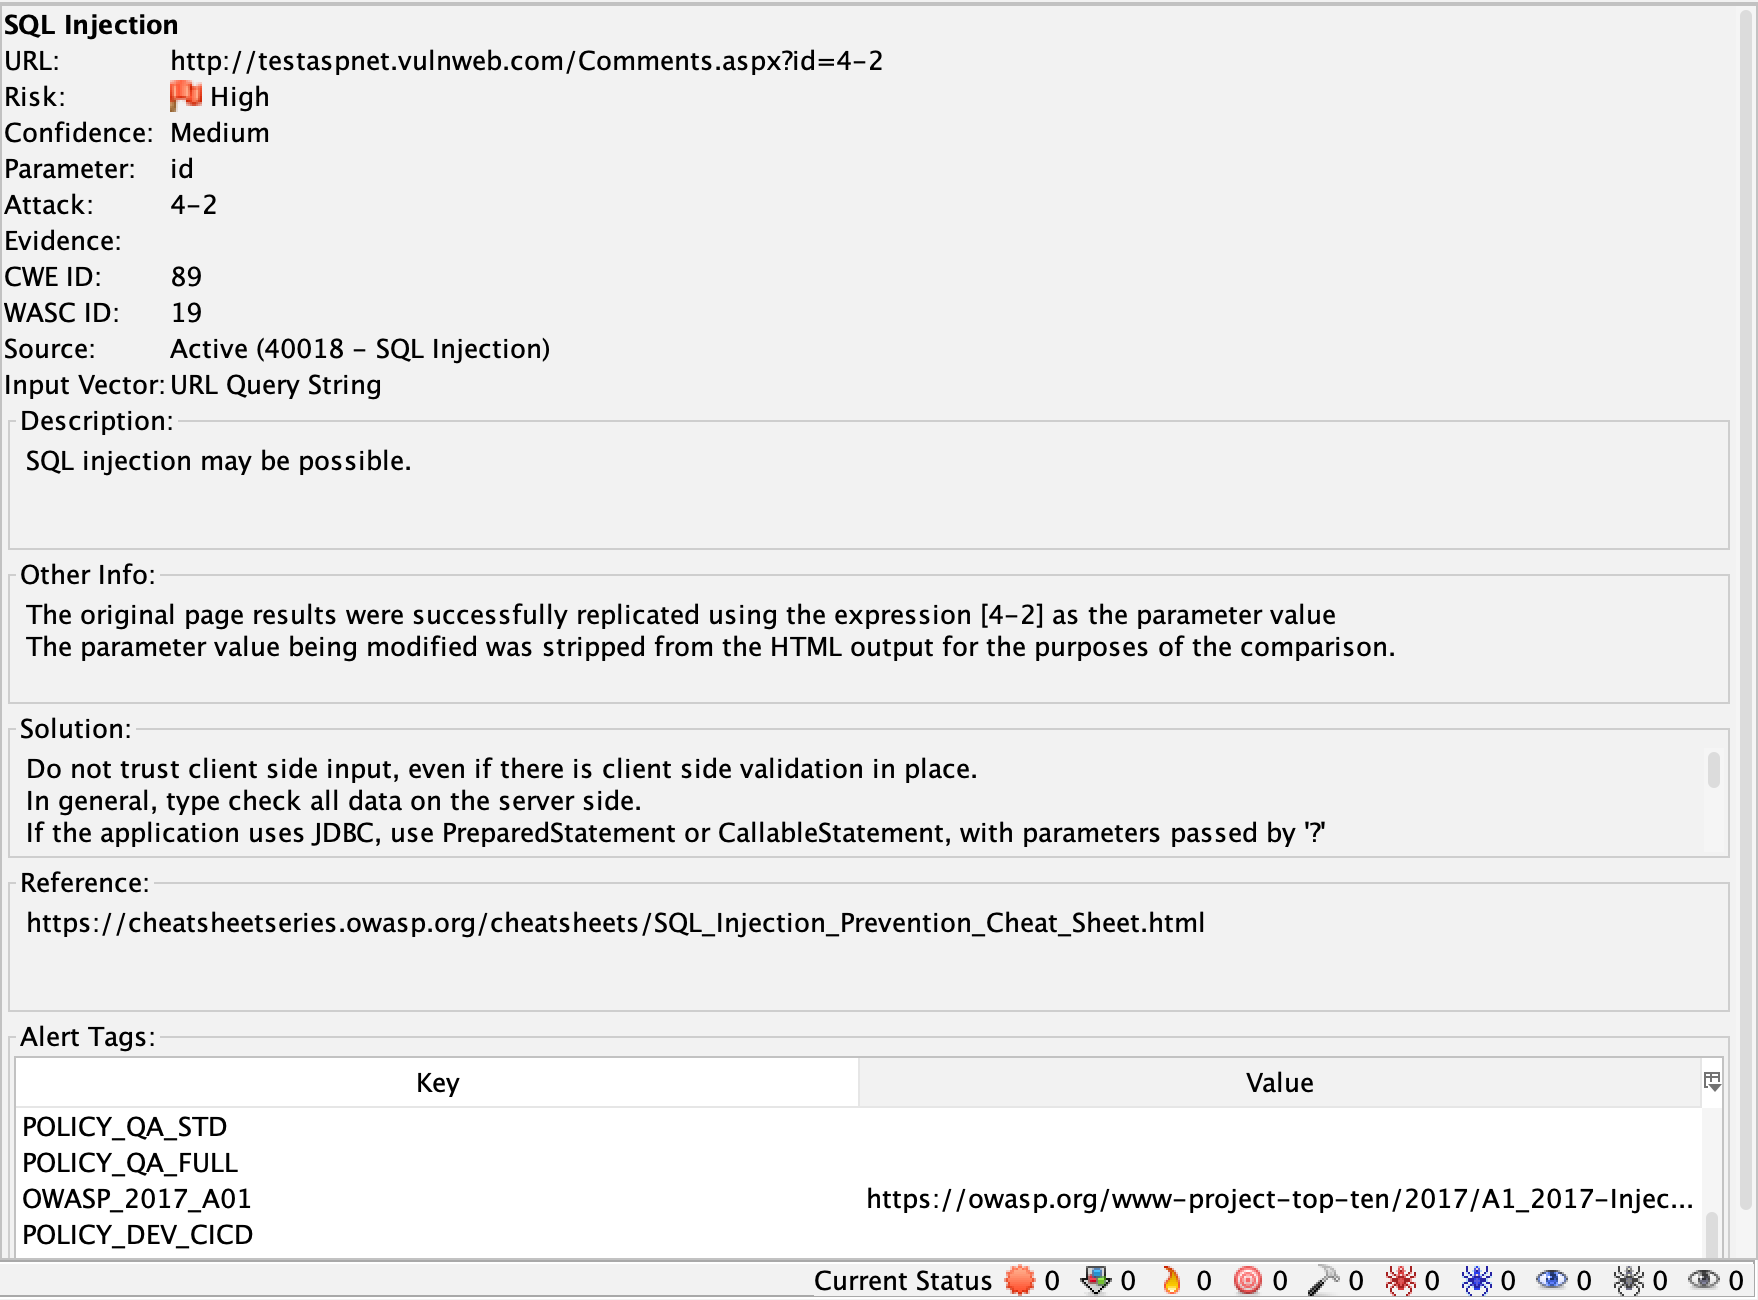
\includegraphics[width=.9\textwidth]{2}
\end{center}

Суть уязвимости заключается в том, что веб-приложение не корректно обрабатывает входящий параметр id (id=4-2) в URL и позволяет злоумышленнику внедрять пользовательский ввод напрямую в SQL-запрос, что может привести к исполнению произвольного SQL-кода на сервере базы данных.
Уязвимости CWE-89.

\begin{center}
  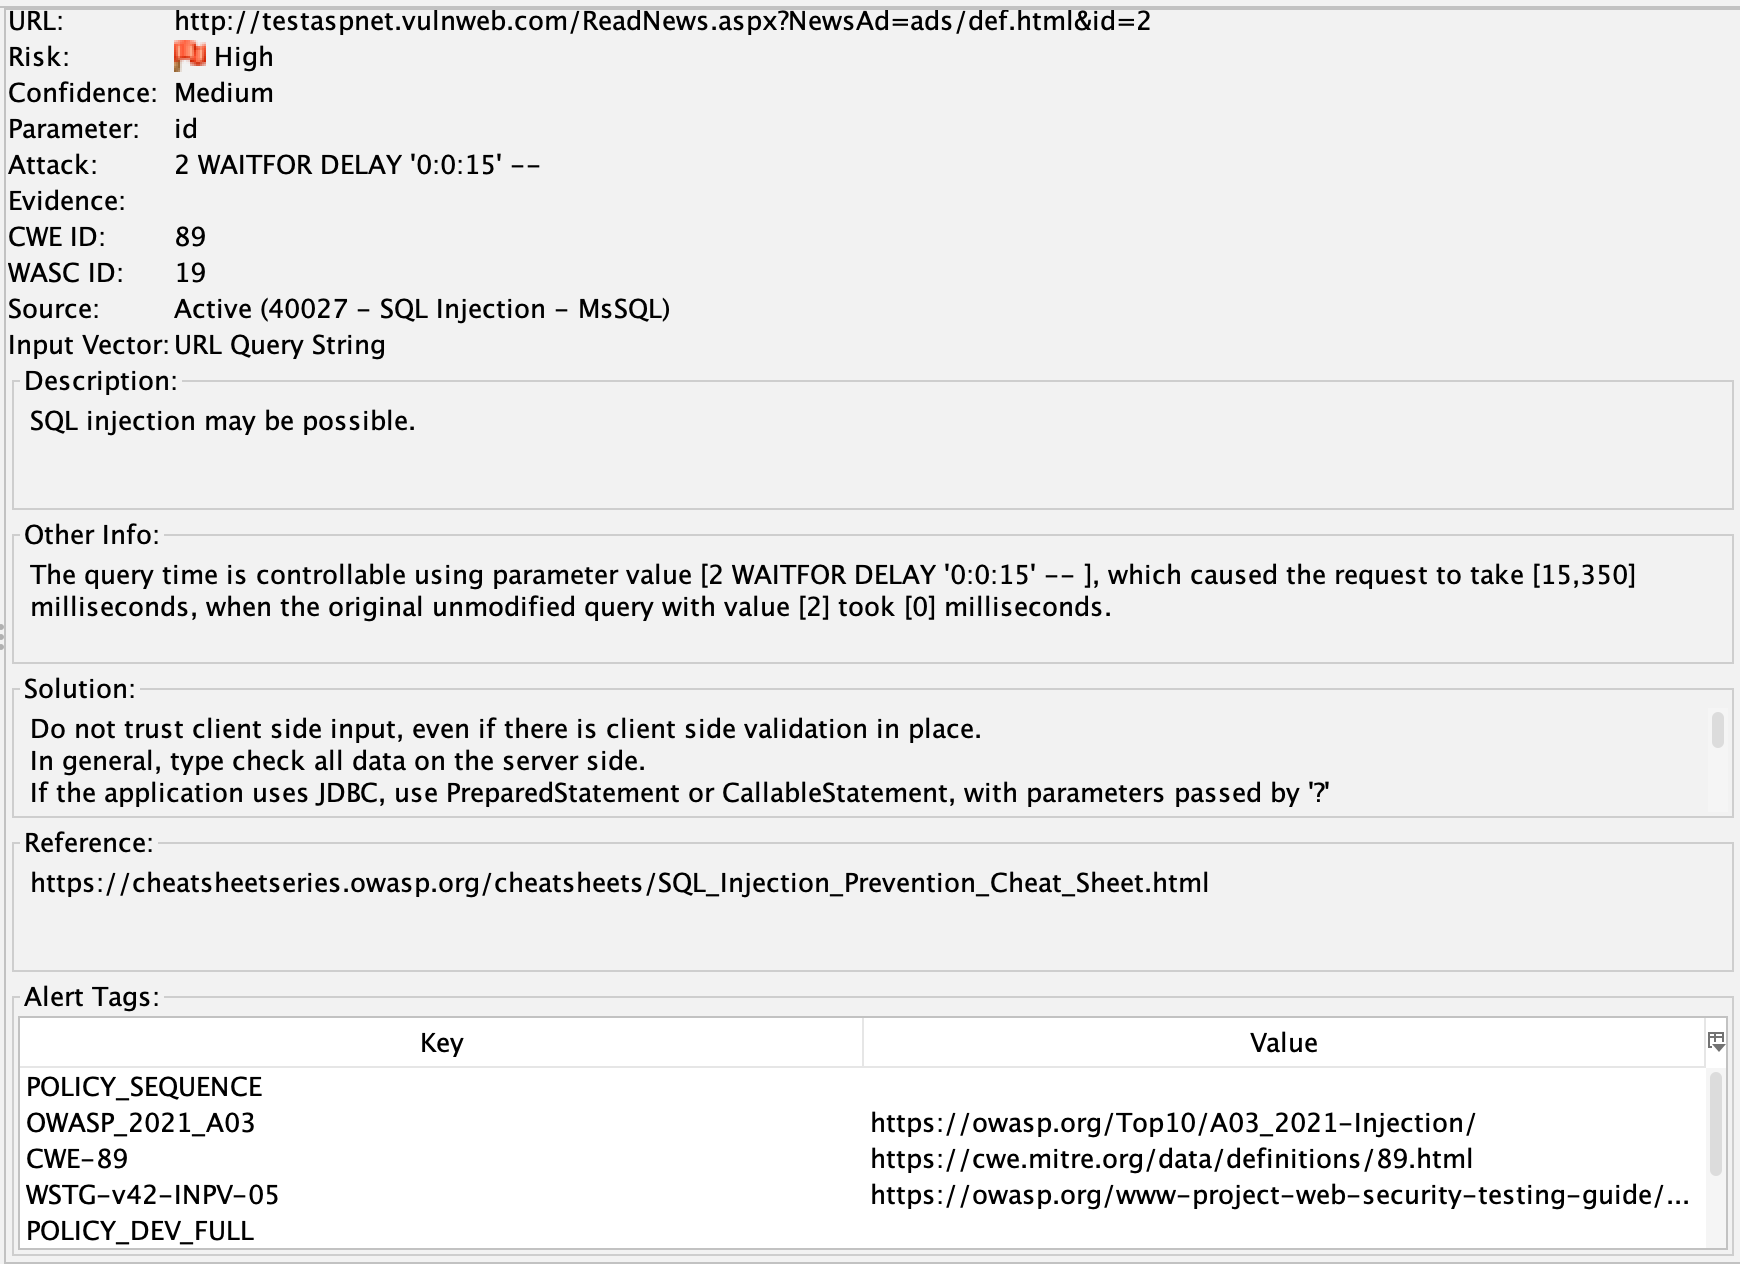
\includegraphics[width=.9\textwidth]{3}
\end{center}

Такой же тип уязвимости SQL Injection, подтверждённая использованием конструкции:

\begin{lstlisting}
  id=2 WAITFOR DELAY '0:0:15'--
\end{lstlisting}

Значение параметра id, переданного через строку запроса, не фильтруется должным образом. Злоумышленник смог внедрить SQL-команду WAITFOR DELAY, что привело к искусственной задержке обработки запроса на сервере (на 15 секунд).
Уязвимости CWE-89.

\section{Absence of Anti-CSRF Tokens}

\begin{center}
  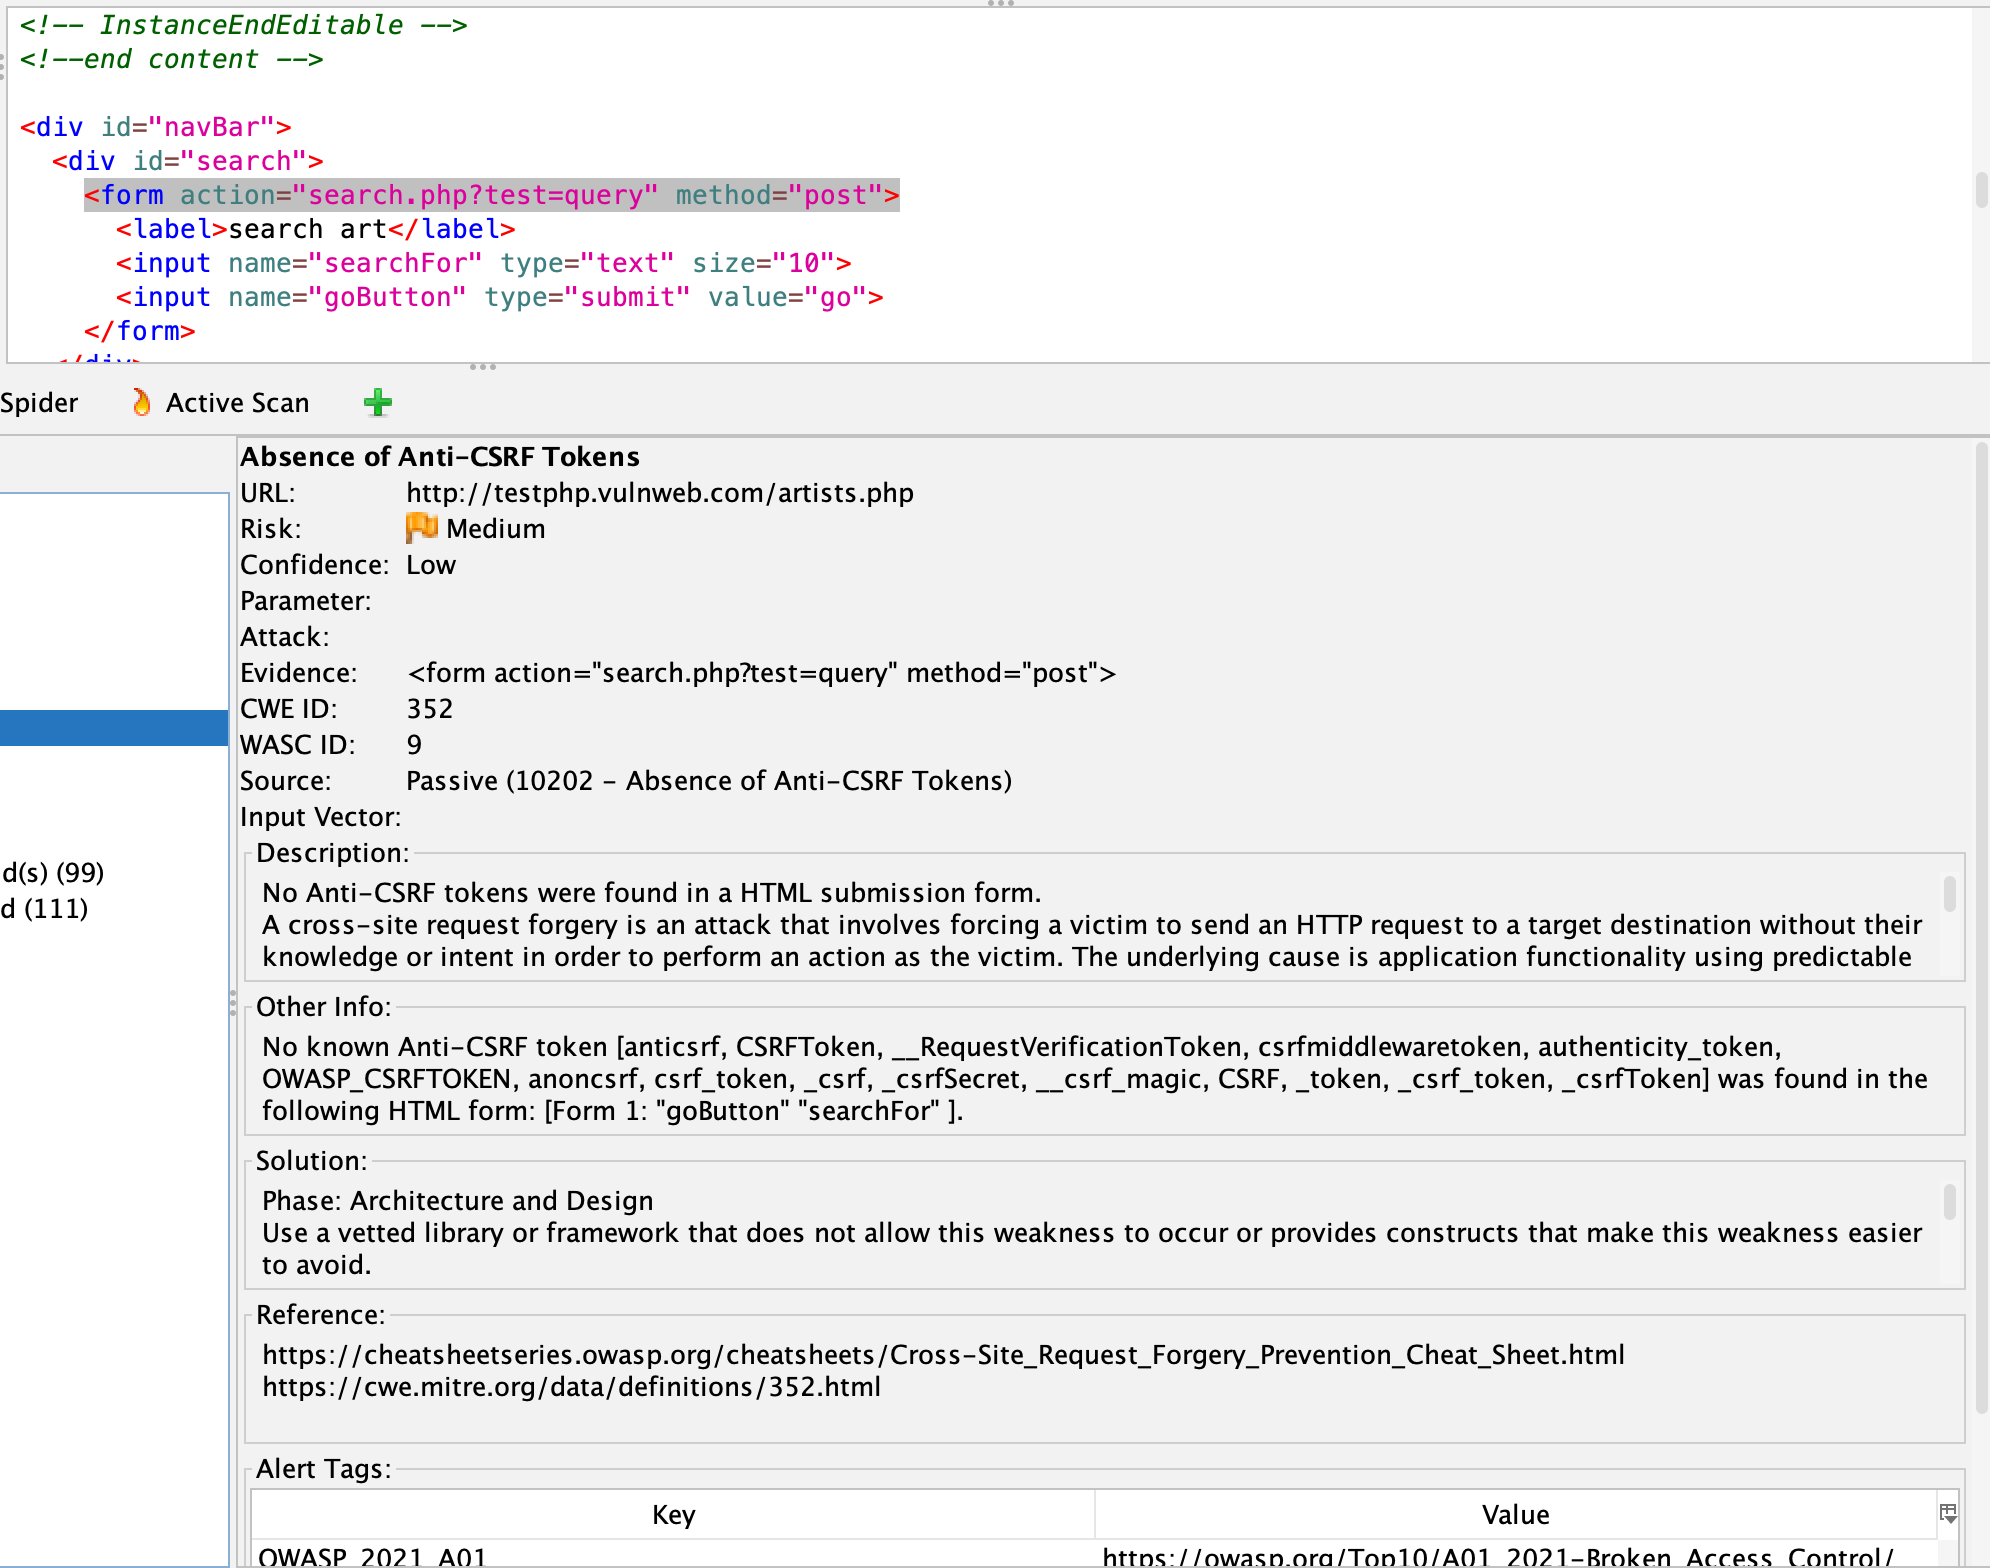
\includegraphics[width=.9\textwidth]{5}
\end{center}

Выявлена уязвимость Absence of Anti-CSRF Tokens в HTML-форме. Это означает, что при отправке формы на сервер не используется уникальный токен, предотвращающий межсайтовые подделки запросов (CSRF).
Злоумышленник может заставить пользователя выполнить нежелательное действие на сайте от его имени, подделав POST-запрос, так как форма не содержит анти-CSRF токена. При отсутствии такого токена сервер не может отличить легитимный запрос пользователя от сгенерированного злоумышленником, что позволяет атаки типа CSRF.
Уязвимости CWE-352.

\section{Content Security Policy (CSP) Header Not Set}
\begin{center}
  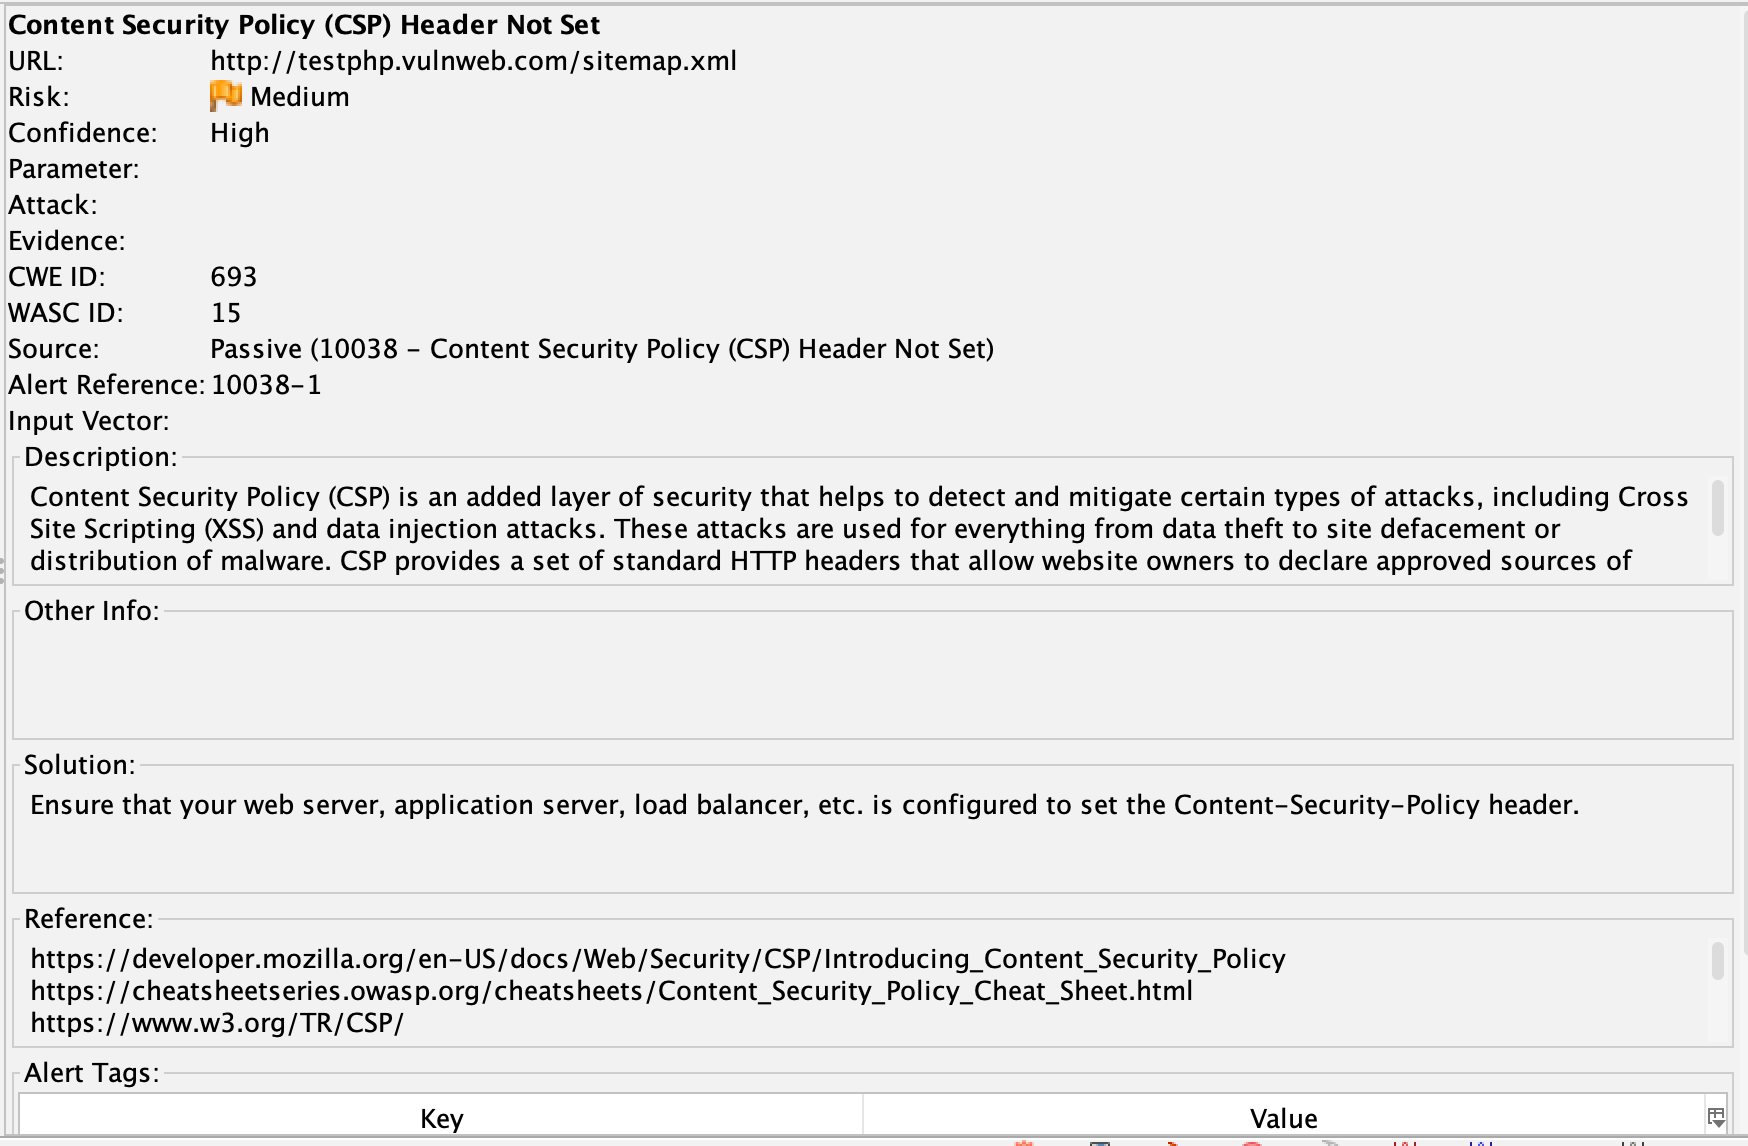
\includegraphics[width=.9\textwidth]{6}
\end{center}
CSP — это дополнительный уровень безопасности веб-приложений, который позволяет ограничить источники исполнения скриптов, стилей и других ресурсов на сайте. При отсутствии этого заголовка сайт становится более уязвимым к атакам типа XSS (межсайтовый скриптинг) и инъекциям данных.
Уязвимости CWE-693.

\section*{Результаты}

Освоил базовые навыки динамического тестирования безопасности (DAST) на
примере тестового приложения http://testaspnet.vulnweb.com.


\end{document}

\begin{center}
  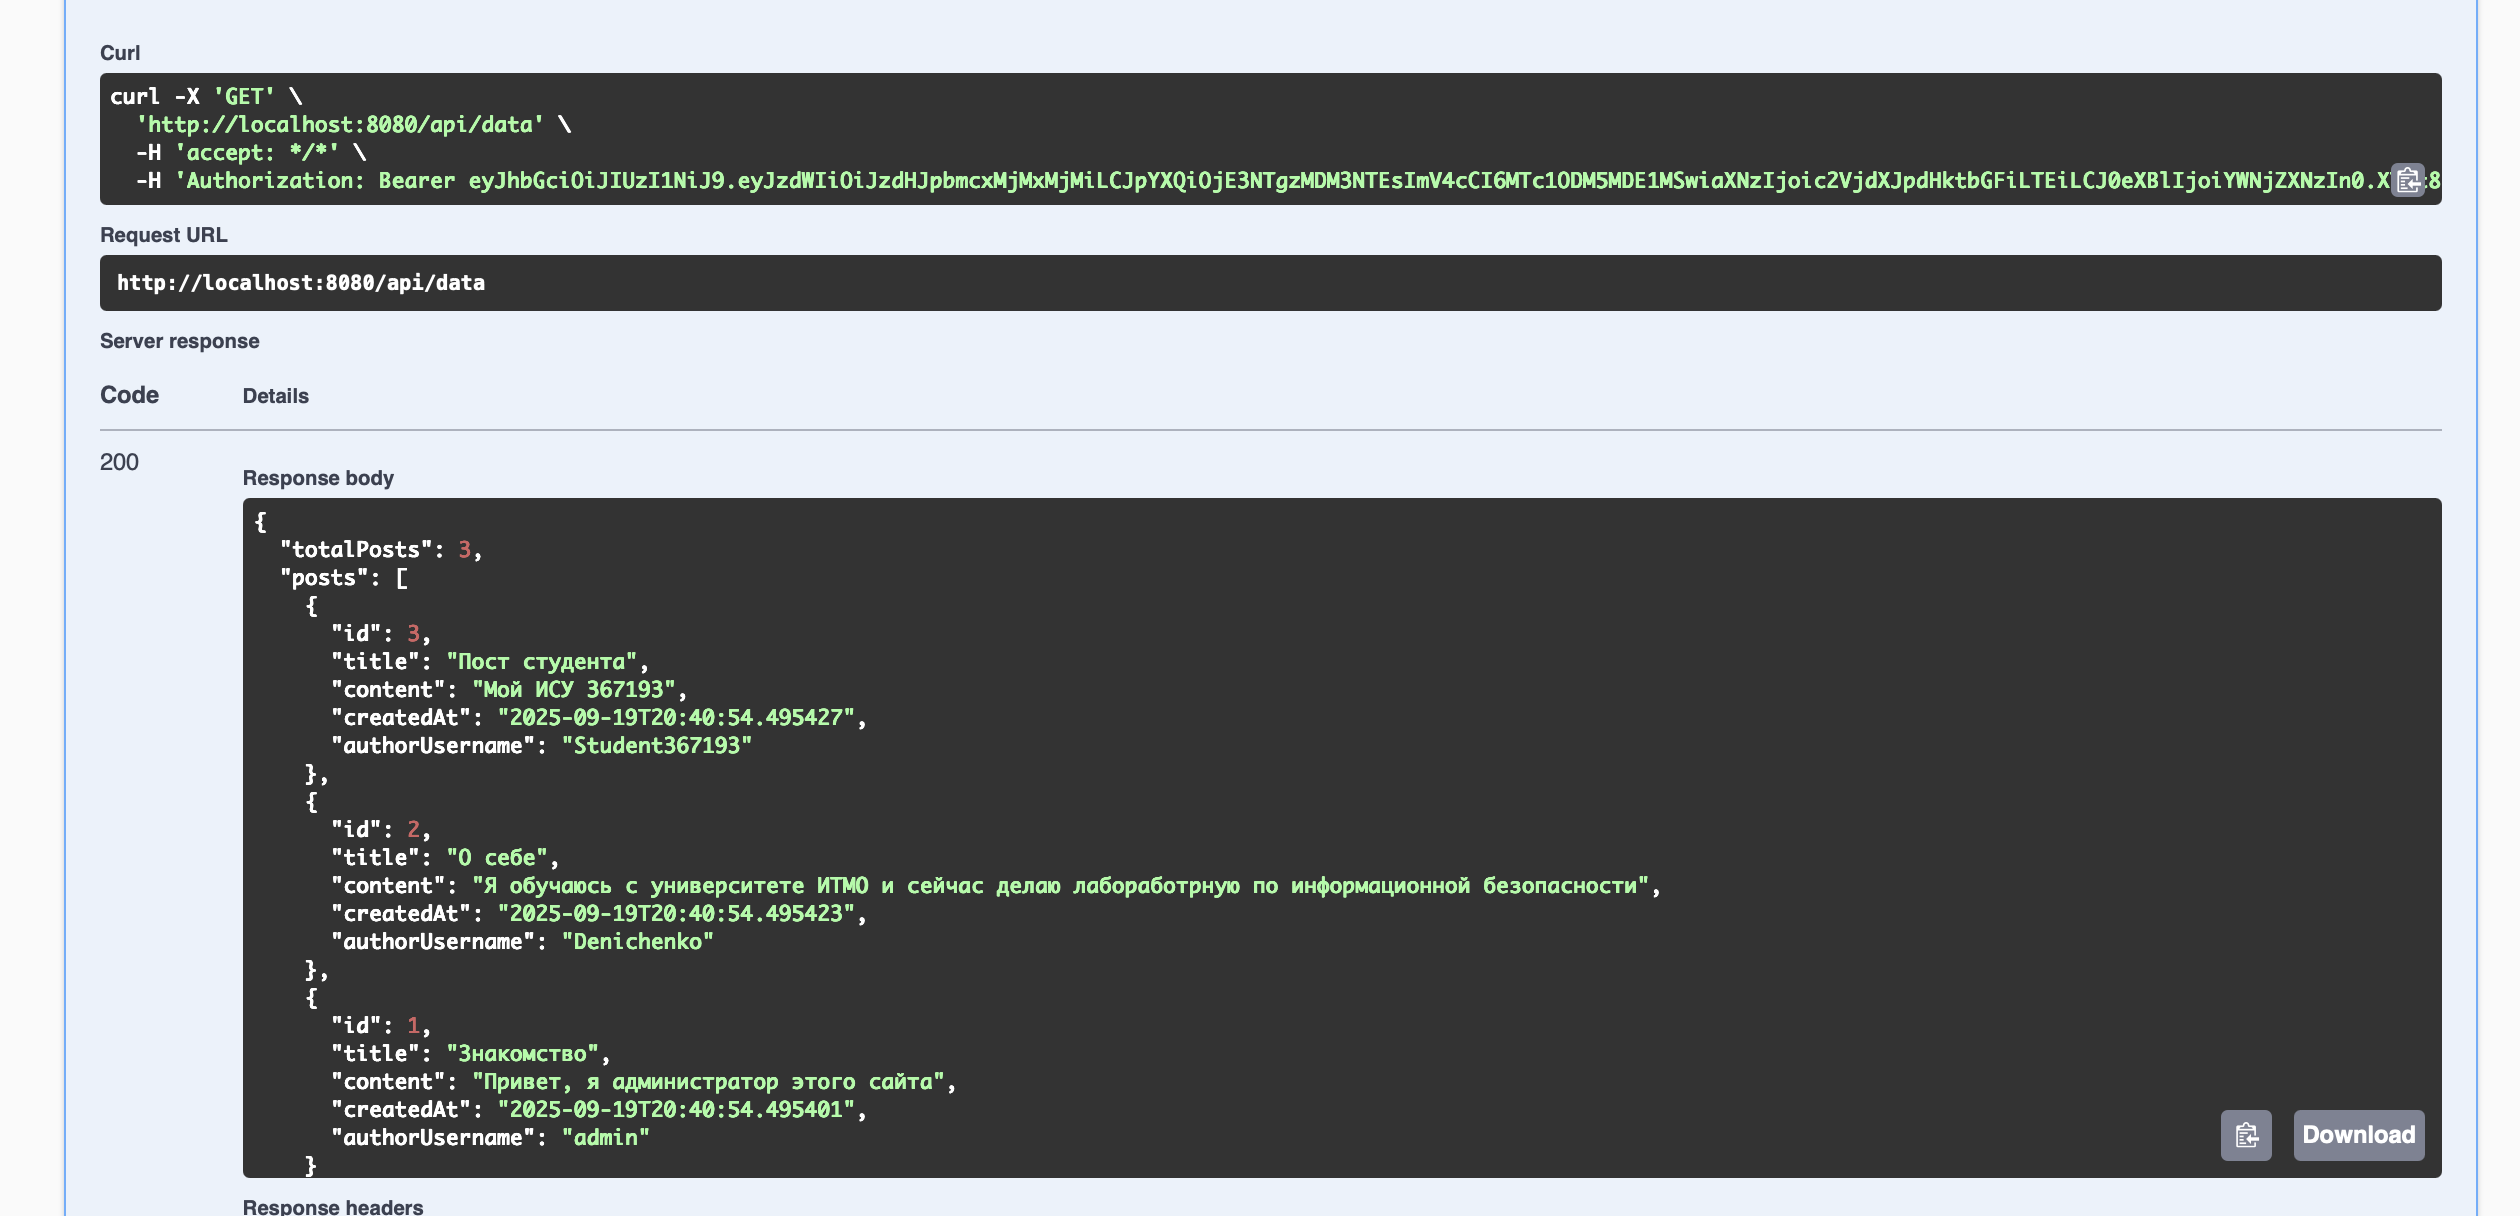
\includegraphics[width=.9\textwidth]{posts}
\end{center}

\href{https://github.com/Alex-de-bug/security-lab-1/actions/runs/17864752066}{Последний верный CI} (https://github.com/Alex-de-bug/security-lab-1/actions/runs/17864752066)
